\documentclass[12pt]{article}
\usepackage[english]{babel}
\usepackage[utf8x]{inputenc}
\usepackage{amsmath}
\usepackage{graphicx}
\usepackage[colorinlistoftodos]{todonotes}
\usepackage{array}
\usepackage{multirow}
\usepackage{tabularx}
\usepackage{gensymb}

\begin{document}

% Title page template downloaded from: 
% https://www.overleaf.com/latex/examples/title-page-with-logo/hrskypjpkrpd

%\documentclass[12pt]{article}
%\usepackage[english]{babel}
%\usepackage[utf8x]{inputenc}
%\usepackage{amsmath}
%\usepackage{graphicx}
%\usepackage[colorinlistoftodos]{todonotes}

%\begin{document}

\begin{titlepage}

\newcommand{\HRule}{\rule{\linewidth}{0.5mm}} % Defines a new command for the horizontal lines, change thickness here

\center % Center everything on the page
 
%-----------------------------------------------------------------------------------
%	HEADING SECTIONS
%-----------------------------------------------------------------------------------

\includegraphics[width=\columnwidth]{Images/PU1linehighres.png}\\[1cm]
%\textsc{\LARGE Princeton University}\\[1.5cm] % Name of your university/college
\textsc{\Large MAE 322: Mechanical Design}\\[0.5cm] % Major heading such as course name
\textsc{\large Spring 2019}\\[1cm] % Minor heading such as course title

%-----------------------------------------------------------------------------------
%	TITLE SECTION
%-----------------------------------------------------------------------------------

\HRule \\[0.6cm]
{ \huge \bfseries Final Design Report}\\[0.4cm] % Title of your document
\HRule \\[1cm]

{\Large May 14, 2019}\\[2cm] % Date, change the \today to a set date if you want to be precise

 
%-----------------------------------------------------------------------------------
%	Team Info
%-----------------------------------------------------------------------------------

{\large \textbf{Team:} The SaRRchaeologists}\\[1cm]
{\large \textbf{Robot:} DynaSaRR}\\[1.6cm]

\begin{minipage}[t]{0.4\textwidth}
\begin{flushleft} \large
\emph{Submitted By:}\\
Jackson Artis\\
Morgan Baker\\
Sam Dale\\
Alexandra Koskosidis\\
Evan Quinn\\
Alex Rogers
\end{flushleft}
\end{minipage}
~
\begin{minipage}[t]{0.4\textwidth}
\begin{flushright} \large
\emph{Submitted To:} \\
Prof. Daniel Nosenchuck\\
Glenn Northey\\
Al Gaillard\\
Aaron Goodman\\
\end{flushright}
\end{minipage}\\[1cm]

\vfill % Fill the rest of the page with whitespace

\end{titlepage}


%\end{document}
%{\Large \textbf{Team Roles}}

\addcontentsline{toc}{section}{Team Roles}
\section*{Team Roles}

% \begin{minipage}[t]{0.4\textwidth}
%     \begin{itemize}
%     \item Column 2 content 1
%     \item Column 2 content 2
%     \end{itemize}
%   \end{minipage}

\begin{center}
\resizebox{\textwidth}{!}{
\begin{tabular}{ |c|c|c|c| } 
    \hline
    Name & Specialty & Responsibilities & PDR Contributions \\
    \hline
    Jackson Artis & CAD Work & cell3 & cell4\\
    \hline
    Morgan Baker & Machining & cell3 & cell4\\
    \hline
    Sam Dale & Coding & cell3 & cell4\\
    \hline
    Alexandra Koskosidis & Team Leader, Analysis & cell3 & cell4\\
    \hline
    Alex Rogers & CNC & cell3 & cell4\\
    \hline
    Evan Quinn & Electrical Engineering & cell3 & cell4\\
    \hline
    
\end{tabular}}
\end{center}

\vfill % Fill the rest of the page with whitespace
\newpage

\section{Executive Summary}
The SaRRchaeologists are building a Search and Rescue Robot (SaRR) meant to successfully navigate a course with challenges resembling those a SaRR responding to the September 11th attacks may have faced. These challenges include manually navigating to and picking up a medical kit weighing 3 pounds, autonomously traversing a wall 1 foot in height, autonomously navigating a narrow chute, and finally, autonomously placing a medical kit in a basket identified by a bright light. \\

Holding true to the original intent of the assignment, The SaRRchaeologists wanted to build a robot that could genuinely be used for Search and Rescue missions. As such, modularity and robustness were held as the primary concerns during this design and manufacturing process. A premium was placed on the ability to quickly modify the robot to handle any unforeseen obstacles along the course, as well as its ability to withstand strong impulses and large drops. Additionally, in order to differentiate itself from other SaRRs, DynaSaRR was also designed to solve these challenges in an innovative way.\\

The primary mechanism, the lifting arm, utilizes carefully analyzed geometry in order to handle the task at hand. The arm rotates and raises the front portion of DynaSaRR, while the rear wheel drive propels the robot atop the first step. The lifting arm then continues to rotate, dropping DynaSaRR on the step. This process is repeated for the next step. As DynaSaRR dismounts from the wall, the combination of the angled front wheels, shock absorbing springs, and force distributing frame will all work in unison to lessen the effect of the sudden impact when hitting the ground. \\

The DynaSaRR represents the result of careful planning and attention to detail. Its design allows it to handle many precarious scenarios without taking damage, and it can easily be modified to adapt to different obstacles and tasks. As a result, it is exactly the kind of SaRR that an individual or organization would want to perform the assigned tasks.


\newpage


\tableofcontents
\newpage


\section{Introduction}

The objective of this project was to design and manufacture a Search and Rescue Robot (SaRR) capable of navigating an obstacle course in order to deliver a first aid kit (a.k.a. med-kit) to a simulated victim. The obstacle course consists of a pylon, a 1-foot tall wall, and a chute. The first portion of the course involves picking up the med-kit, navigating the pylon, and approaching the wall. This portion will be completed using open-loop drive control of the SaRR via an RC controller. However, the rest of the course must be completed autonomously by the SaRR. The closed-loop portion of the course has three unique components to be traversed by the SaRR. First, the SaRR must cross a wall (one foot tall by three feet wide and consisting of two equally sized steps). The SaRR then approaches and navigates through a chute without hitting the sides. Finally, the SaRR must acquire and track a light signal in order to deposit the med-kit in a basket. \\

While the SaRR design was influenced largely by the task of overcoming the wall obstacle, issues of maneuverability and speed, for the sake of the remainder of the obstacle course, were still taken into account. The major component for handling the wall obstacle is a wall-traversal arm (a.k.a. the lifting arm). The arm is designed to prop the front wheels up onto the first step, then rotate around fully and push the front wheels onto the top of the wall. The arm will rotate again, helping to pull the robot over the wall. In order to reduce the strain on the SaRR as it lands on the far side of the wall, the front wheels are held by forks which are connected to the chassis by shock-absorbing springs. The other component that had a large impact on the design was the mechanism for the collection of the med-kit. It was designed to not only allow for secure pick-up and easy drop off, but also allow for the center of mass adjustment if necessary.  \\

Preliminary design was centered around studying videos of past SaRRs, both successful and unsuccessful alike. From these videos, the SaRRchaeologists were able to conclude that a simple med-kit gripper design consisting of a V-shaped protrusion on a rotating arm would be successful in picking up and depositing the med-kit. A visual of the medical kit arm can be seen in the appendix as figure 8. It was also clear, however, that the inclusion of a bracket to hold the med-kit in place during the course would be necessary in order to prevent it from being dislodged. Special attention was paid to the SaRRs that were able to get their front half over the wall, but then either became stuck or toppled forward or backward. In response to this issue, the SaRRcheaologists' lifting arm was designed to continue to push the SaRR over the wall should it become stuck at the top, while also preventing it from rotating backwards. Moreover, rear wheel drive coupled with the front arms made sure it would not stall atop the second step. What's more, the front wheel forks were placed at an angle to prevent the apparatus from toppling forward upon impact with the ground. \\

The SaRRcheaologists sought to design a SaRR that could not only complete the aforementioned tasks, but could do so in an interesting and innovative way that was not reliant overly complex and failure-prone mechanisms. By iterating through many different geometries for the chassis, front fork assembly, and lifting arm, a simple, yet innovative design was achieved. In order to maintain the maneuverability of the SaRR, the width and length of the chassis would need to be balanced properly. The chassis would need to be wide enough to hold various required mechanisms, and needed to be short enough to prevent the chassis from reaching precarious angles at the peak of the wall. Additionally, a large emphasis was placed on using wheels with enough traction and height to aid the SaRR in getting over the wall when working in concert with the lifting arm. Finally, there are a few aspects of the design that serve to increase the robustness of the SaRR. First, the chassis frame will be built of 80/20 aluminum extrusion which will double as a base to which various components will be bolted. The T-slotted 80/20 frame also serves the purpose of making the SaRR modular, as parts can be replaced and configurations altered with ease. Second, the front forks are mounted on shock-absorbing springs in order to reduce the impact when the front half comes over the wall. Finally, small tires were chosen as rear wheels so that any impact as the back end falls from the wall would be properly absorbed. \\

For visual representations, please refer to Figs. 1, 4, and 9.

\begin{figure}[H]
    \centering
    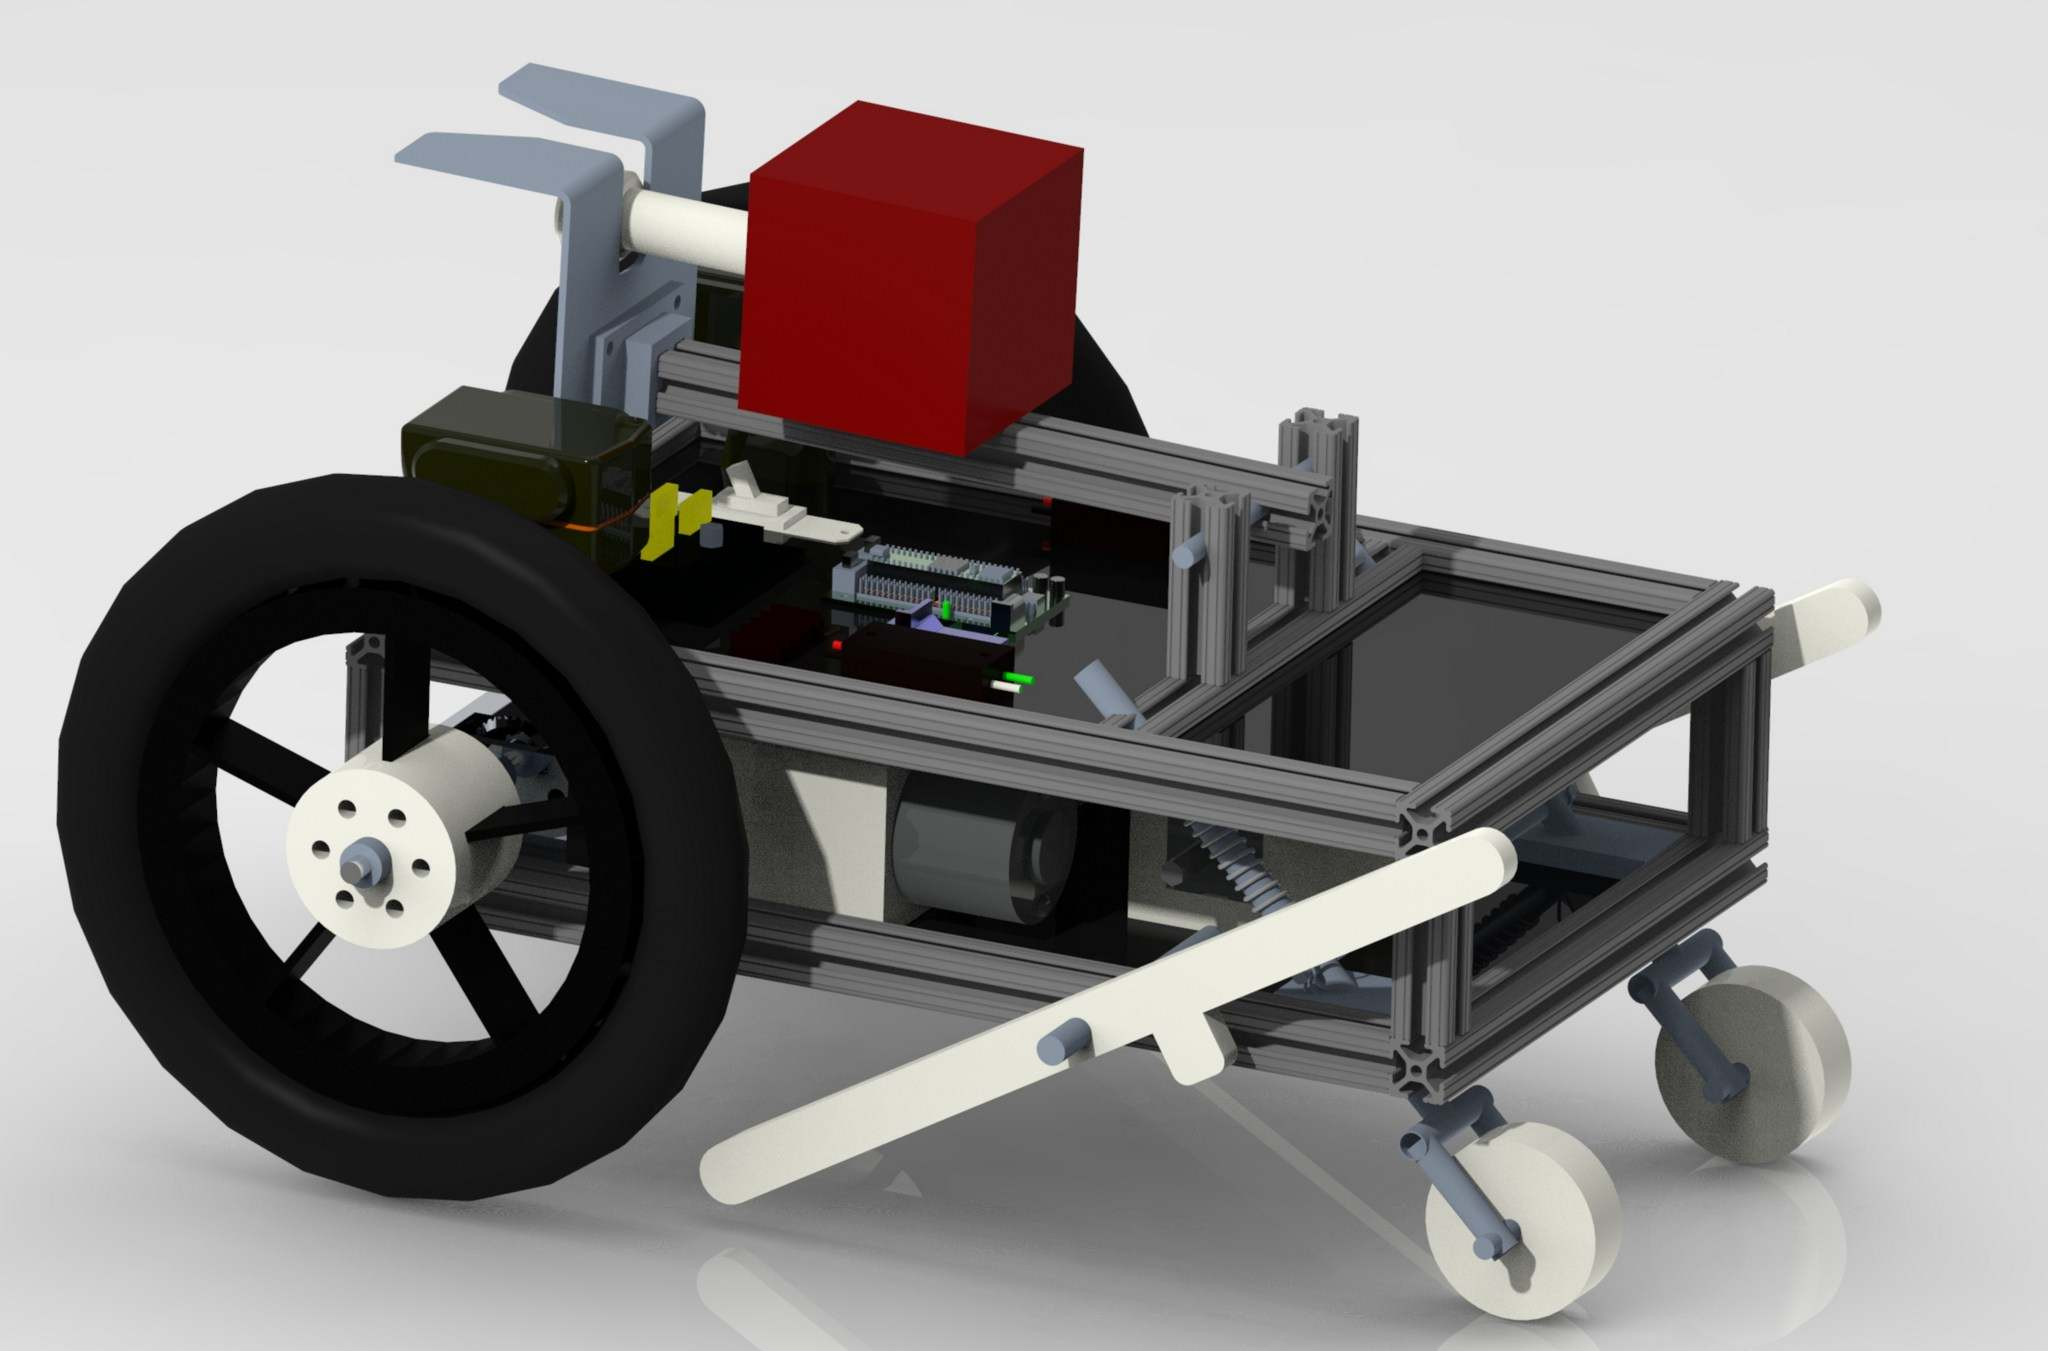
\includegraphics[width=1.1\linewidth]{PreliminaryDesignReport/55939435_166367590950985_2070774621560373248_n.png}
    \caption{DynaSaRR Schematic}
    \label{fig:my_label}
\end{figure}




\section{Specifications}
\subsection{Size, Weight, Speed}
Below is a list of design specifications that we have selected for our SaRR. Drive wheels with a 12 inch diameter were chosen, which are larger than those used in the original in-class model; these are composed of rubber, inflatable tires for enhanced control while navigating. This design choice will also reduce slippage and ensure that more torque from the motor is being utilized than if tires with less traction were used, increasing speed on the ground and obstacle climbing ability. DynaSaRR was also extended in length relative to the sample robot in order to accommodate our lifting arm mechanism, which will help DynaSaRR to successfully navigate the wall obstacle.  \\
The weight of the SaRR was estimated using material assignment features inside of CREO 5.0 and density calculations made for the materials the team already possessed, such as the drill batteries, Teensy board and battery storage unit. \\
Additionally, the frame consists of a rectangular prism shape formed by T-slotted 80/20 aluminum 6061 extrusions. This shape allows for maximum organizational efficiency and will allow for the easy mounting of parts and modularity.
\begin{itemize}
\item Total Weight: 50 lbs
\item Frame Width: 12 in
\item Frame Length: 19.5 in
\item Frame Height: 5 in
\item Frame Clearance Height: 3.9 in
\item Drive Wheel Diameter: 12 in
\item Drive Wheel Width: 1.7 in
\item Total SaRR Width: 15 in
\item Total SaRR Length (Lifting Arms Up): 22 in
\item Total SaRR Height: 14 in
\end{itemize}
\\

In order to estimate DynaSaRR's speed along a flat surface, it was first necessary to calculate the total force required to maintain speed:
$$F_{tot} = F_r + F_{drag}.$$
$F_r$ is the rolling resistance, and is calculated as $$F_r = c*W,$$ where $c$ is the rolling resistance coefficient of the tires, and $W = m*g$ is the weight of the robot (mass times acceleration due to gravity). $c$ for bike tires on waxed wood was found to be $0.002$, and on asphalt was $0.005$. From these values, $c$ for our tires on linoleum was estimated be $0.004$. The weight of DynaSaRR was estimated to be 50 lbs., so $F_r$ was calculated as $77.24 \frac{lb*in}{s^2}$.
$$ F_{drag} = \frac{C_d*A* \rho_{air}*V^2}{2}.$$
Here, $C_d$ is the coefficient of drag, which was estimated to be 1.16 due to the ratio of length (20in) to height (12in) of approximately 2 of the robot face (calculated for a flat rectangular plate). $A$, the area of the robot, was calculated as $0.3*20*12$, because the SaRRchaeologists estimated that only about $30 \%$ of the 20 by 12 rectangle actually contained material. $\rho_{air} = 4.06*10^-5 \frac{lb}{in^3}$, and $V$ is the velocity of the robot. In order to complete the calculations, the velocity had to be estimated and then the following calculations had to be iterated over until the estimated and calculated velocities matched (detailed calculations are shown in the Appendix). In the final iteration, a velocity of 7mph was assumed, so $F_{drag}$ was calculated as $25.763 \frac{lb*in}{s^2}$. Thus, $F_{tot} = 102.97 \frac{lb*in}{s^2}$. From this, torque was calculated as 
$$ \tau = r_{wheel}*F_{tot}*sin( \theta).$$
Since this calculation is for a flat surface, $\theta = 90 \degree $, and the wheels have a radius of 12 in. Drivetrain efficiency was estimated to be $84.1 \%$, so actual torque for each driven wheel (2) was calculated as
$$ \tau_{real} = \frac{\tau}{2*0.841} = 367.33 \frac{lb*in^2}{s^2}.$$
This was then multiplied by a safety factor of 2 and converted to Newton-meters, resulting in a torque of $0.22 N*m$. The corresponding RPM (read off Fig. 2) at that torque was 4700 rpm, which was converted to a speed by multiplying by the wheel circumference, resulting in a speed estimate of 6.99mph--extremely close to the original estimate. This showed that this iteration of calculations would be an accurate predictor of DynaSaRR's performance: it is expected to travel at approximately 7mph.

\begin{figure}[H]
    \centering
    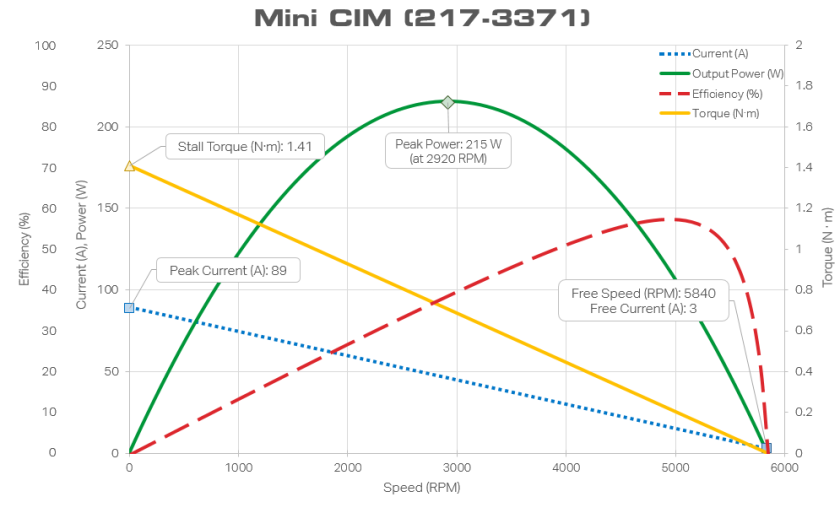
\includegraphics[width=1.1\linewidth]{PreliminaryDesignReport/mini-cim-motor-curve-20151207.png}
    \caption{Motor Curves for the VEX Motors}
    \label{fig:my_label}
\end{figure}

The DynaSaRR has an estimated top speed of 7.2 mph or 10.56 feet per second. Additionally, the turning radius was calculated to be 19.6 in. As such, moving at top speed, it would take the DynaSaRR approximately 10 seconds to complete the entire course, with the exception of the wall traversal portion. With the estimate of 1 minute for wall traversal (see page 10 calculations and expectations), together, the SaRRchaeologists predict that it will take approximately 3 minutes to complete the course (as an additional 1 minute and 50 seconds was added to the additional 10 second prediction to account for lessened driving speed, medical kit acquiring, and unforeseen hangups). \\



\subsection{Operational and Navigational Modes}
The SaRR will have two modes of control, one which is open-loop and will be controlled by inputs to a controller, and one which is autonomous and will be operated by closed-loop Arduino code sent to a Teensy board. The open-loop navigation will be used to locate and retrieve the med kit, then move to the front of the wall obstacle. \\

In order to successfully navigate to the med kit, grasp the med kit, and then traverse to the front of the wall obstacle, the open-loop remote controller (the human-technology interface in this design) has 4 directional inputs: forward, backward, right turn and left turn. The controller also has 2 switches which amplify an isolated channel based on the location of the corresponding knob located on the controller. One of these switch/knob combinations is to trigger the lifting and lowering of the med kit retrieval arm, and the other is used to engage the autonomous mode of the robot. The signals from the remote controller are obtained on the SaRR by a wireless receiver and are read into the Teensy microcontroller where actions are assigned based on the values transmitted.  In open-loop mode, these are the only inputs that will be received by the SaRR.\\

When the right shoulder switch is flipped, the value of the designated channel will be higher than a certain threshold. While this is true, the SaRR will be in autonomous mode. In autonomous mode, the only inputs to the microcontroller are from three proximity sensors and two light sensors. One proximity sensor will be located on the front of the SaRR, and the other two will each be located on opposite sides of the frame. The two light sensors will be located on the underside of the frame and will be facing forward. \\When in autonomous mode, the SaRR will have to complete four tasks: cross over the wall, navigate the chute, find and track the light source, and drop the med kit into the basket. \\

The task of crossing the wall will be completed by the two lifting arms on either side of the frame. These arms will rotate on an axle and be connected to a third motor of output torque ~1.3 Nm. They will have a pre-programmed sequence that will first rotate forward once, an action completed accurately using the speed of the motor at a specified power and a timed action in the code of the sequence. The Teensy will then drive the rear wheels toward the wall at a low speed to achieve maximum torque (~1.3 Nm from motor). The lifting arms will then rotate around once again, pushing off the top of the step and lifting the front wheels over the top of the wall as the rear wheels drive forward, and then will complete a third rotation, latching onto the top of the wall and, with the assistance of the large driving wheels in the rear, levering and pulling the SaRR over the obstacle. The lifting arm rotations sequence will be written into the code and will be adjusted in trials as necessary to obtain successful crossing on every attempt. As soon as the lifting arms are through their final rotation, autonomous chute navigation will be engaged in the Teensy code.\\

The SaRR will then move forward and begin to navigate the chute. This will be done through the use of the proximity sensors on the front, left and right of the frame, providing feedback that will be used to issue instructions to the SaRR that keep it well within the walls of the chute. By using a PID controller within the Arduino code, success will be achieved after some moderate testing and tuning. This closed-loop feedback controller will allow for the most versatile navigation system.
Once through the chute, the SaRR will no longer register a high value from the proximity sensors residing on the side of the frame and will enter detection mode. In this mode, the SaRR will rotate clockwise until the forward-facing light sensors detect the drop zone flashlight. At this point, the robot will move forward, continuously monitoring the strength of the light to ensure it is moving in the right direction. This action will be implemented with ad-hoc code that checks the values of the light sensors and adjusts accordingly. Once the SaRR is close to the drop zone, a very high reading on the front-mounted proximity sensor will cause the SaRR to stop and lower the med kit arm, dropping the med kit into the target.\\


\section{Detailed Design and Analysis}

Free-body analysis of DynaSaRR in various stages of the obstacle course is shown in Figs. 3-5.

\begin{figure}[H]
    \centering
    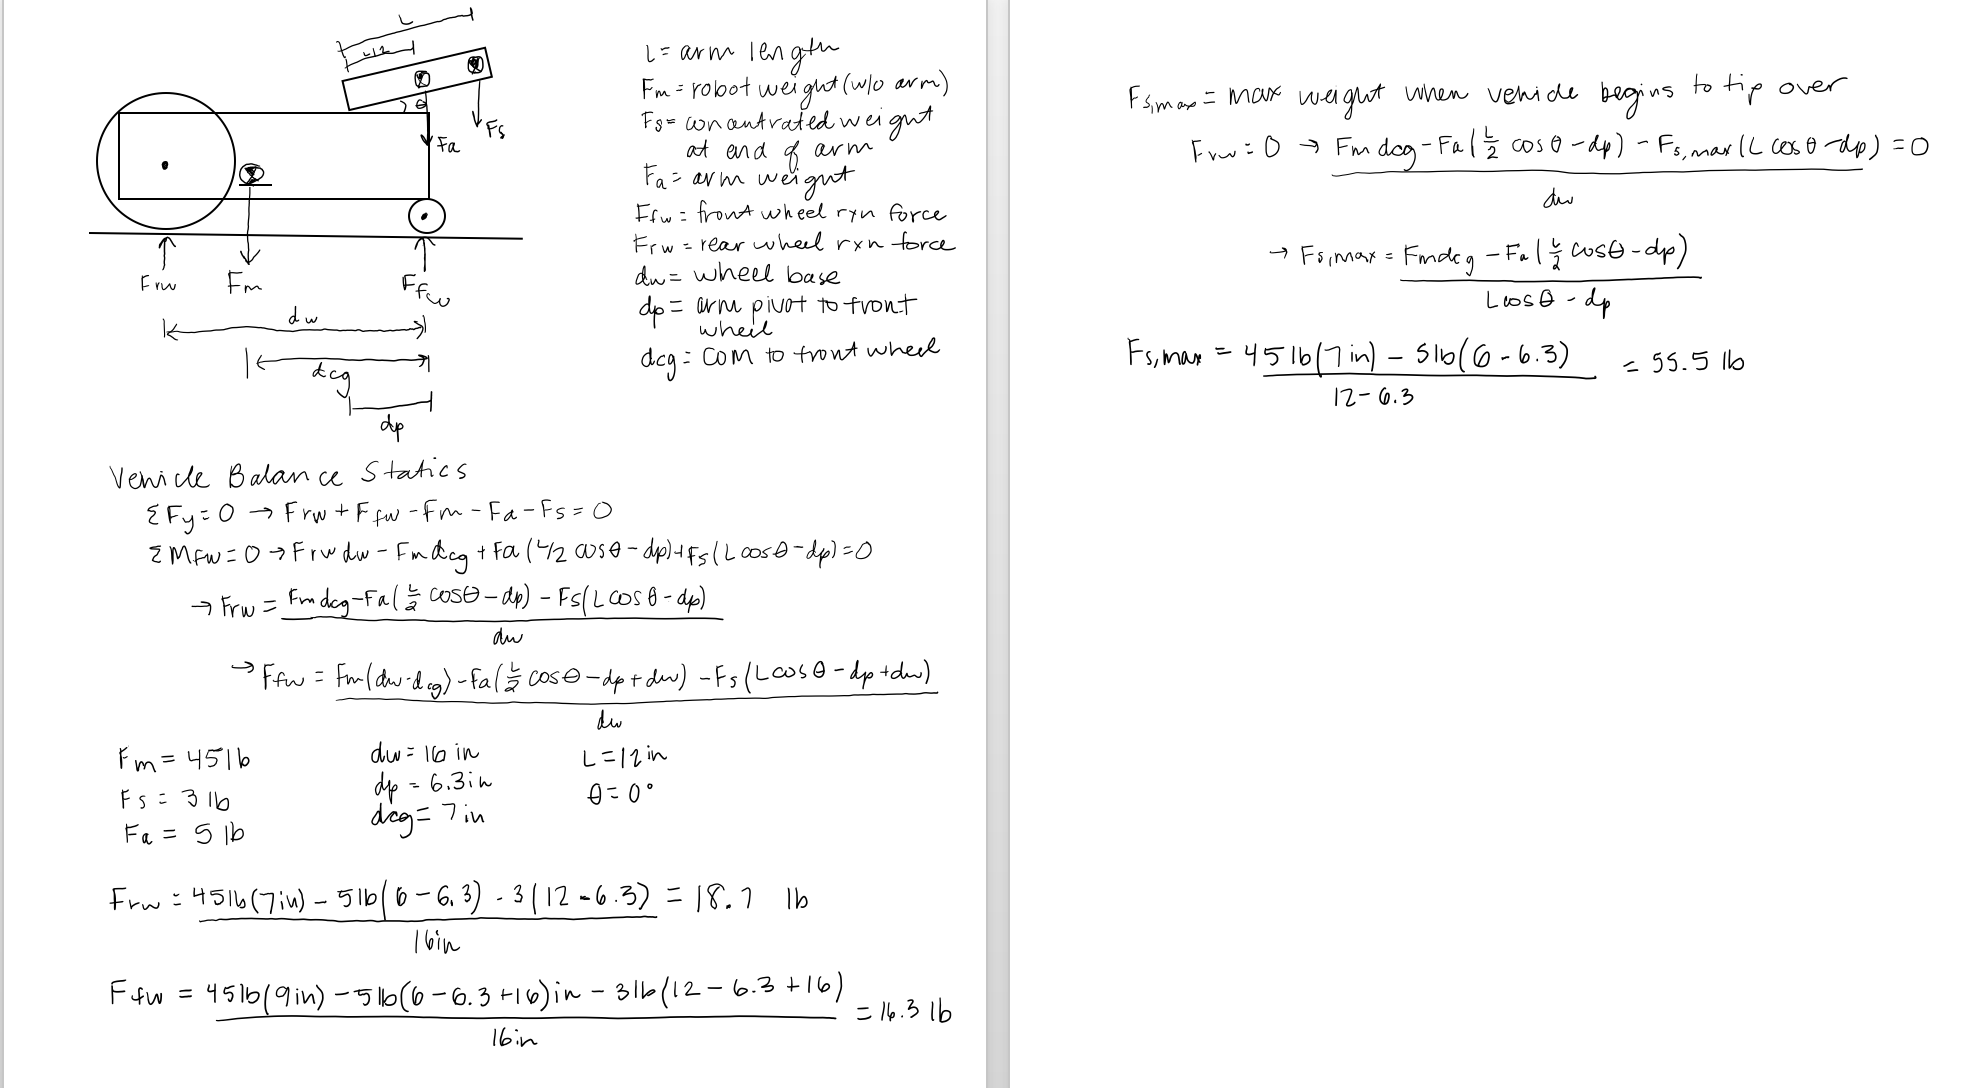
\includegraphics[width=1.2\linewidth]{PreliminaryDesignReport/1.png}
    \caption{Free Body Diagrams and Calculations for DynaSarr During Med-Kit Retrieval}
    \label{fig:my_label}
\end{figure}

\begin{figure}[H]
    \centering
    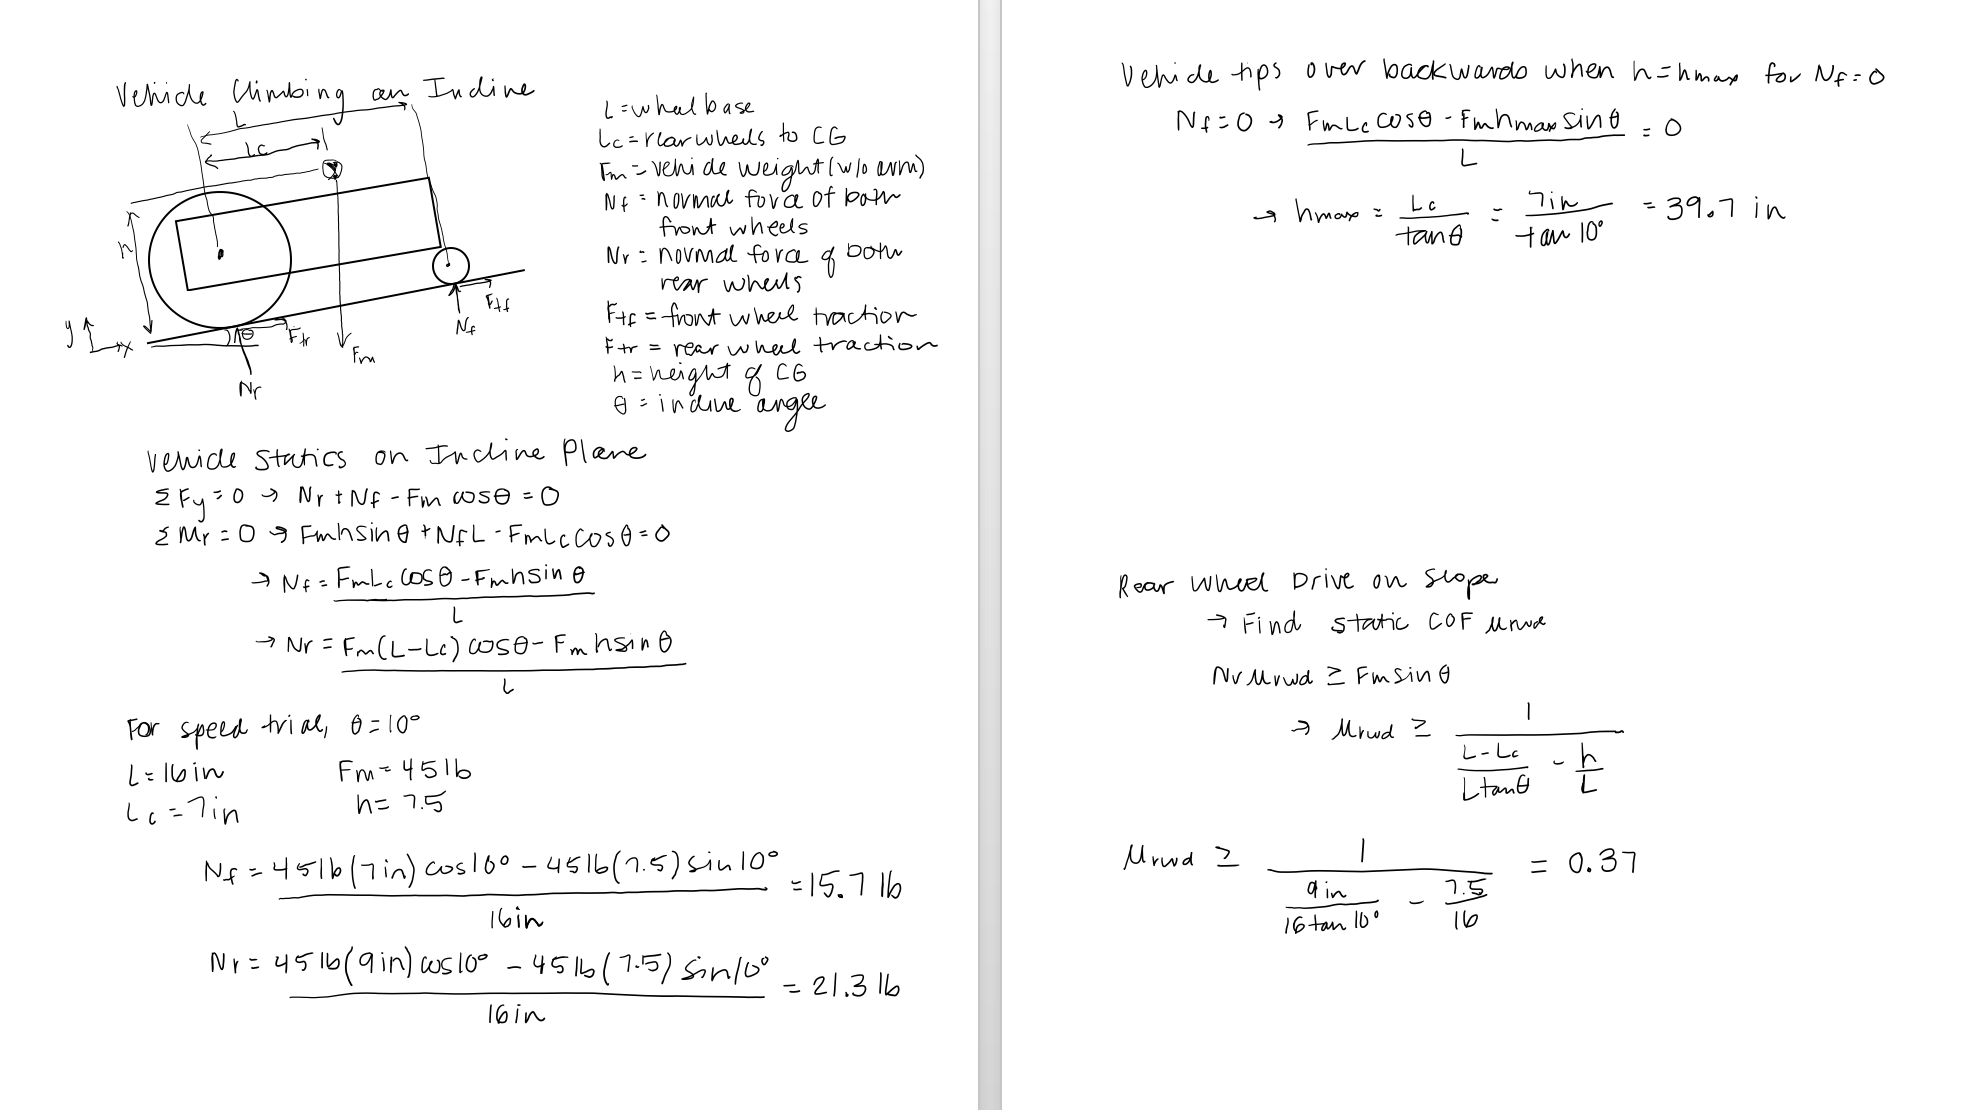
\includegraphics[width=1.2\linewidth]{PreliminaryDesignReport/2.png}
    \caption{Free Body Diagrams and Calculations for DynaSarr On An Incline}
    \label{fig:my_label}
\end{figure}

\begin{figure}[H]
    \centering
    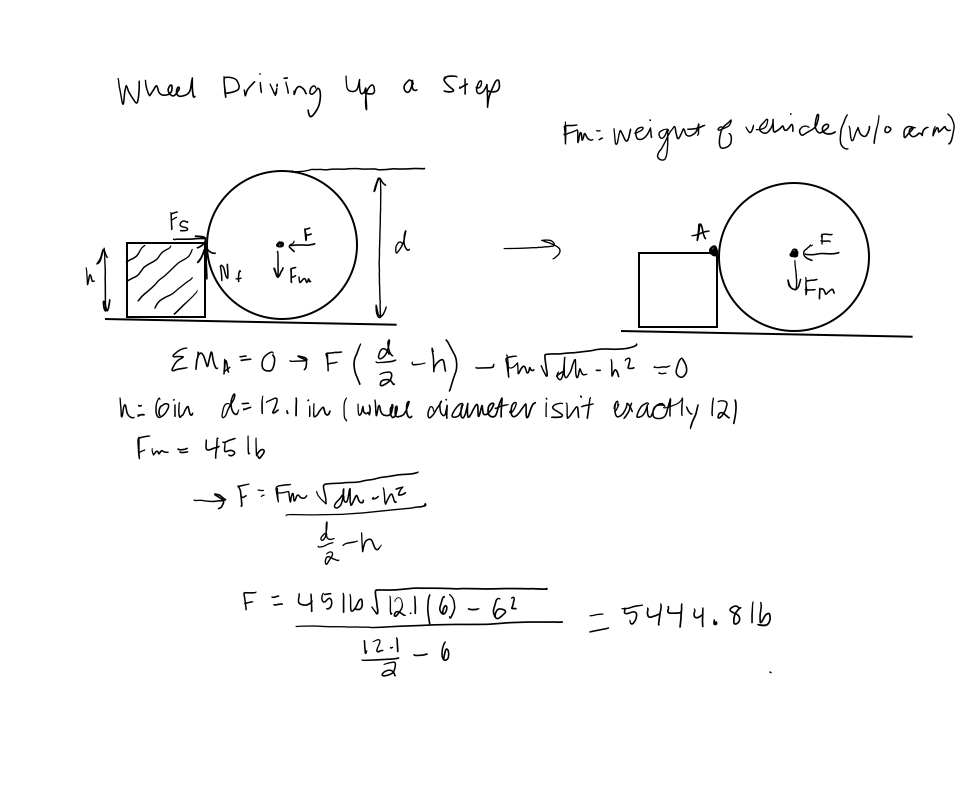
\includegraphics[width=1.1\linewidth]{PreliminaryDesignReport/3.png}
    \caption{Free Body Diagrams and Calculations for DynaSarr Driving Up a Step}
    \label{fig:my_label}
\end{figure}

In designing a med-kit retrieval mechanism, the primary considerations were a gripper that would not require tremendous precision in order to pick up the med-kit handle, and a mechanism to lock the med-kit into place after it was lifted onto the SaRR, so that it would not fall out during the wall traversal or other sections of the obstacle course. To fit the first consideration, DynaSaRR will lower an arm with a flat gripper component at the front. The gripper will be composed of two triangular pieces of aluminum to funnel the handle of the med-kit into the triangular space between them and then into a slot cut into the gripper. The V-shaped gripper is intended to minimize the precision required in driving up to the med-kit by providing a larger capture area than just a small slot the side of the handle. The arm will then rotate upward, with the med-kit pivoting in the gripper slot until it falls into a bracket mounted on the underside of the arm to keep it from falling out.

The SaRRchaeologists decided to utilize the same Mini CIM Motor for the lifting arm as is used for the back wheels. The published data has a stall torque of 1.41 Newton-Meters. The SaRRchaeologists used a conservative estimate of 1.3 Newton-Meters, a gear ratio of 24:1, and equation (1) 
\begin{equation}
    torque_{new} = torque_{original} * gearRatio
\end{equation}

and where able to achieve a theoretical torque of 31.2 newton-meters. This value is equivalent to 23.08 foot-pounds of generated torque. 

The SaRRchaeologists assumed that at the inital step, in order for the front wheels to be lifted up, approximately $60\%$ of DynaSaRR's weight will have to be lifted. An overly cautious estimate of 50 pounds (including the medical kit's weight) was used for DynaSaRR's weight, suggesting that the SaRRchaeologists planned to lift 30 pounds. Using a lever arm of 8.5 and equation (2) inches, 

\begin{equation}
    torque_{lifting} = weight_{pounds} * \frac{leverArm_{inches}}{12 inches}
\end{equation}

it was calculated that it would take 21.25 foot pounds to lift the front of DynaSaRR up above. As such, The SaRRchaeologists felt comfortable that the lifting arm mechanism would be functional and successful. 

Using the the published data, The SaRRchaeologists found that an RPM of 58 was associated with the necessary raw torque of the motor, 1.3 newton-meters. Using the 24:1 gearing ratio again and equation (3),

\begin{equation}
    RPM_{new} = \frac{RPM_{original}}{gearRatio} 
\end{equation}


it was calculated that the RPM of the lifting arm would be approximately 4. As such, it would take 50 seconds for the lifting arm to perform two 360 degree turns. The SaRRchaeologists assumed a total time of 1 minute necessary to traverse the wall (deciding to add an additional 10 seconds to account for any unforseen issues or hangups). 

\section{Project Management}
Alexandra Koskosidis: Voted Team Leader\\

    It is the primary responsibility of the Team Leader to direct the individual members of the group and the direction of the project as a whole. The Team Leader works with the members of her group to ensure all necessary tasks are undertaken and completed by delegating sub-projects and setting completion date objectives. She schedules team meetings, poses concerns to the group for discussion, and updates all members on progress.\\
    
Alex Rogers: CNC Specialist\\

    The CNC Specialist is mainly responsible for CNCing all CAD parts by creating mill volumes and designing tool paths. The CNC Specialist works closely with Al to check pieces and reserve space in the CNC. Thus, he is also very involved in the main CAD model, adjusting dimensions of parts and making final assemblies to accommodate design changes. The CNC Specialist also works closely with the Hardware and Manufacturing Specialist in the general manufacturing of the robot due to his understanding of the most updated CAD designs. \\
    
Evan Quinn: Hardware and Manufacturing Specialist\\

    The Hardware and Manufacturing Specialist (HMS) is tasked with connecting motors and other electrical components, as well as soldering and wiring inputs and outputs. The HMS works closely with the Programming Specialist to ensure the functionality of proximity and light sensors. He also works with Glenn to machine aluminum pieces like axles, couplings, gearboxes, and gears.\\
    
Jackson Artis: CAD Specialist, Assistant Leader\\
    
    The CAD Specialist oversees the CREO modeling process, in which design ideas are transformed into CAD models that are easy to be manufactured. The CAD specialist is responsible for making sure the CREO model is in a state that is easily and readily transferable to the manufacturing process. What's more, the CAD specialist is responsible for aiding in and overseeing any simulations that might be necessary to ensure success. \\ 

Morgan Baker: Lead Machinist\\

    The Lead Machinist is responsible for the machining of or the overseeing of all machined parts. The LM works closely with Glenn and Al to ensure that the best possible methods are used to create parts. Since machining must be done correctly to ensure the success of the other areas, she consults many of the other specialists to ensure that the SaRR parts are fully functional.\\
    
Sam Dale: Programming Specialist, CAD Assistant\\

    The programming specialist develops all of the code for the robot to autonomously navigate to the light source in the first milestone and to improve upon this code to navigate through the chute using PID control. The wall traversal will also be automated, possibly using distance sensors to provide feedback. Additionally, the CAD Assistant is responsible for implementing the design plan into practical, producible parts. 
    

\subsection{Schedule and Tasks}

\begin{itemize} 
\item Week of Feb. 25th: Demonstrate Open-Loop Drive-train
\begin{itemize}
\item CNC motor holders, cut axles, assemble belt tighteners (2)
\item Wire breadboard, solder wires (1)
\item Program controller, connect to breadboard (1)
\end{itemize}
\end{itemize}
\begin{itemize}
\item Week of Mar. 4th: Closed-Loop Navigation to Light Source 
\begin{itemize}
\item Attach light and proximity sensors (1)
\item Connect sensors to outputs, read sensors (1/2)
\item Write code, read sensor outputs and respond with motor inputs (4)
\end{itemize}
\end{itemize}
\begin{itemize}
\item Week of Mar. 11th: Finalize Design 
\begin{itemize}
\item Individual brainstorming (2)
\item Idea proposals and deliberation (2)
\item Begin CAD design and cardboard prototyping (3)
\end{itemize}
\end{itemize}
\begin{itemize}
\item Week of Mar. 18th: Spring Break 
\begin{itemize}
\item Complete CAD model (10)
\item Complete Bill of Materials and order parts (4)
\item Determine necessary motor torques/gearing
\end{itemize}
\end{itemize}
\begin{itemize}
\item Week of Mar. 24th: Begin Assembly (PDR due 3/29)
\begin{itemize}
\item Manufacture gearbox components (6)
\item Calculations for COM, torque, energy, etc. (6)
\item Complete PDR (3)
\end{itemize}
\end{itemize}
\begin{itemize}
\item Week of Apr. 1st: Speed Trials 
\begin{itemize}
\item Assemble chassis (4)
\item Build gearbox, mount motors, connect wheels (10)
\item Attach and secure hardware
\end{itemize}
\end{itemize}
\begin{itemize}
\item Week of Apr. 8th: Open-Loop Wall Traversal  
\begin{itemize}
\item Finalize and machine lifting arms (4)
\item Mount lifting motor, couple axle (1)
\item Program controller, connect to motor input (2)
\end{itemize}
\end{itemize}
\begin{itemize}
\item Week of Apr. 15th: Open-Loop Object Retrieval/Placement  
\begin{itemize}
\item Machine med-kit arm, connect axle (4)
\item Mount and attach med-kit motor (1)
\item Program controller, connect to motor output (2)
\end{itemize}
\end{itemize}
\begin{itemize}
\item Week of Apr. 22nd: Closed-loop Chute Traversal  
\begin{itemize}
\item Mount, calibrate additional proximity sensors (3)
\item Write code for wall detection (6)
\item Program autonomous mode, adjust sensitivity (4)
\end{itemize}
\end{itemize}
\begin{itemize}
\item Week of Apr. 29th: Design Adjustments   
\begin{itemize}
\item Increase overall robustness for drop test (4)
\item Optimize COM (4)
\end{itemize}
\end{itemize}
\begin{itemize}
\item Week of May 6th: Finalization/Relaxation
\begin{itemize}
\item Ideally a stress free week (0)
\item Otherwise, fix what needs fixing (?)
\end{itemize}
\end{itemize}
\begin{itemize}
\item Week of May 13th: Showtime  
\begin{itemize}
\item Demonstration of search and rescue capabilities of DynaSaRR
\end{itemize}
\end{itemize}

\subsection{Management Approach}

The team recognizes that the most important part of the project is constant, effective communication. Before any design or manufacturing began, the group set up a chat on Facebook Messenger, which allows all members to collaborate at the same time from their phone or laptop, and actively identify who has seen the messages and who has not (unlike text message). Furthermore, a WhenIsGood form was compiled to identify the time slots during which each team member would be available. This form makes it very easy for the Team Leader to organize team meetings and assign work to people by the hour. Team meetings are scheduled during the Lab period every Monday, which is considered the Team Lab Time. Any other meetings are scheduled as needed. On each Monday, the team discusses the plan for the week; tasks to tasks to be done, their priority level, who is to work on them, and when each member has the time to work. Each group member also posts their weekly availability in the Facebook group message during this time. Often, sports practices, club meetings, and other conflicts can make it challenging to find a time when all members are available at the same time outside of Monday, but members will frequently meet in smaller groups while working. All members log their hours after any time spent working on the project. The Time Sheet includes a description of the task worked on, which allows the Team Leader to keep track of who is on top of their assignments and who might be behind, as well as a tally of total hours spent by each member. This holds people accountable for the work they have been assigned and agreed to complete. The Milestone schedule is posted in the team chat so everyone knows when certain goals must be reached. All members were present for all Program Management lectures, and a list of "excuses" and unforeseen issues was created; techniques were discussed to deal with them. For example, the constant communication about scheduling and availability was intended to thwart anyone missing a work period because they forgot or were unaware, and the prioritized to-do list shared with all team members was made so that no one would be waiting for another teammate to tell them what the next task to be accomplished should be. Manufacturing errors were predicted to cause some the most challenging set backs. To alleviate these issues, we tried to employ the buddy system, whereby a partner would provide a "sanity check" before anyone attempted to manufacture a part. By taking a couple extra moments to check, the team avoided much longer setbacks trying to re-manufacture or re-order parts. While team dinners have been difficult to schedule, we plan to have one on Nassau Street in the coming week to decompress!

\section{Appendix}


\begin{figure}[H]
    \centering
    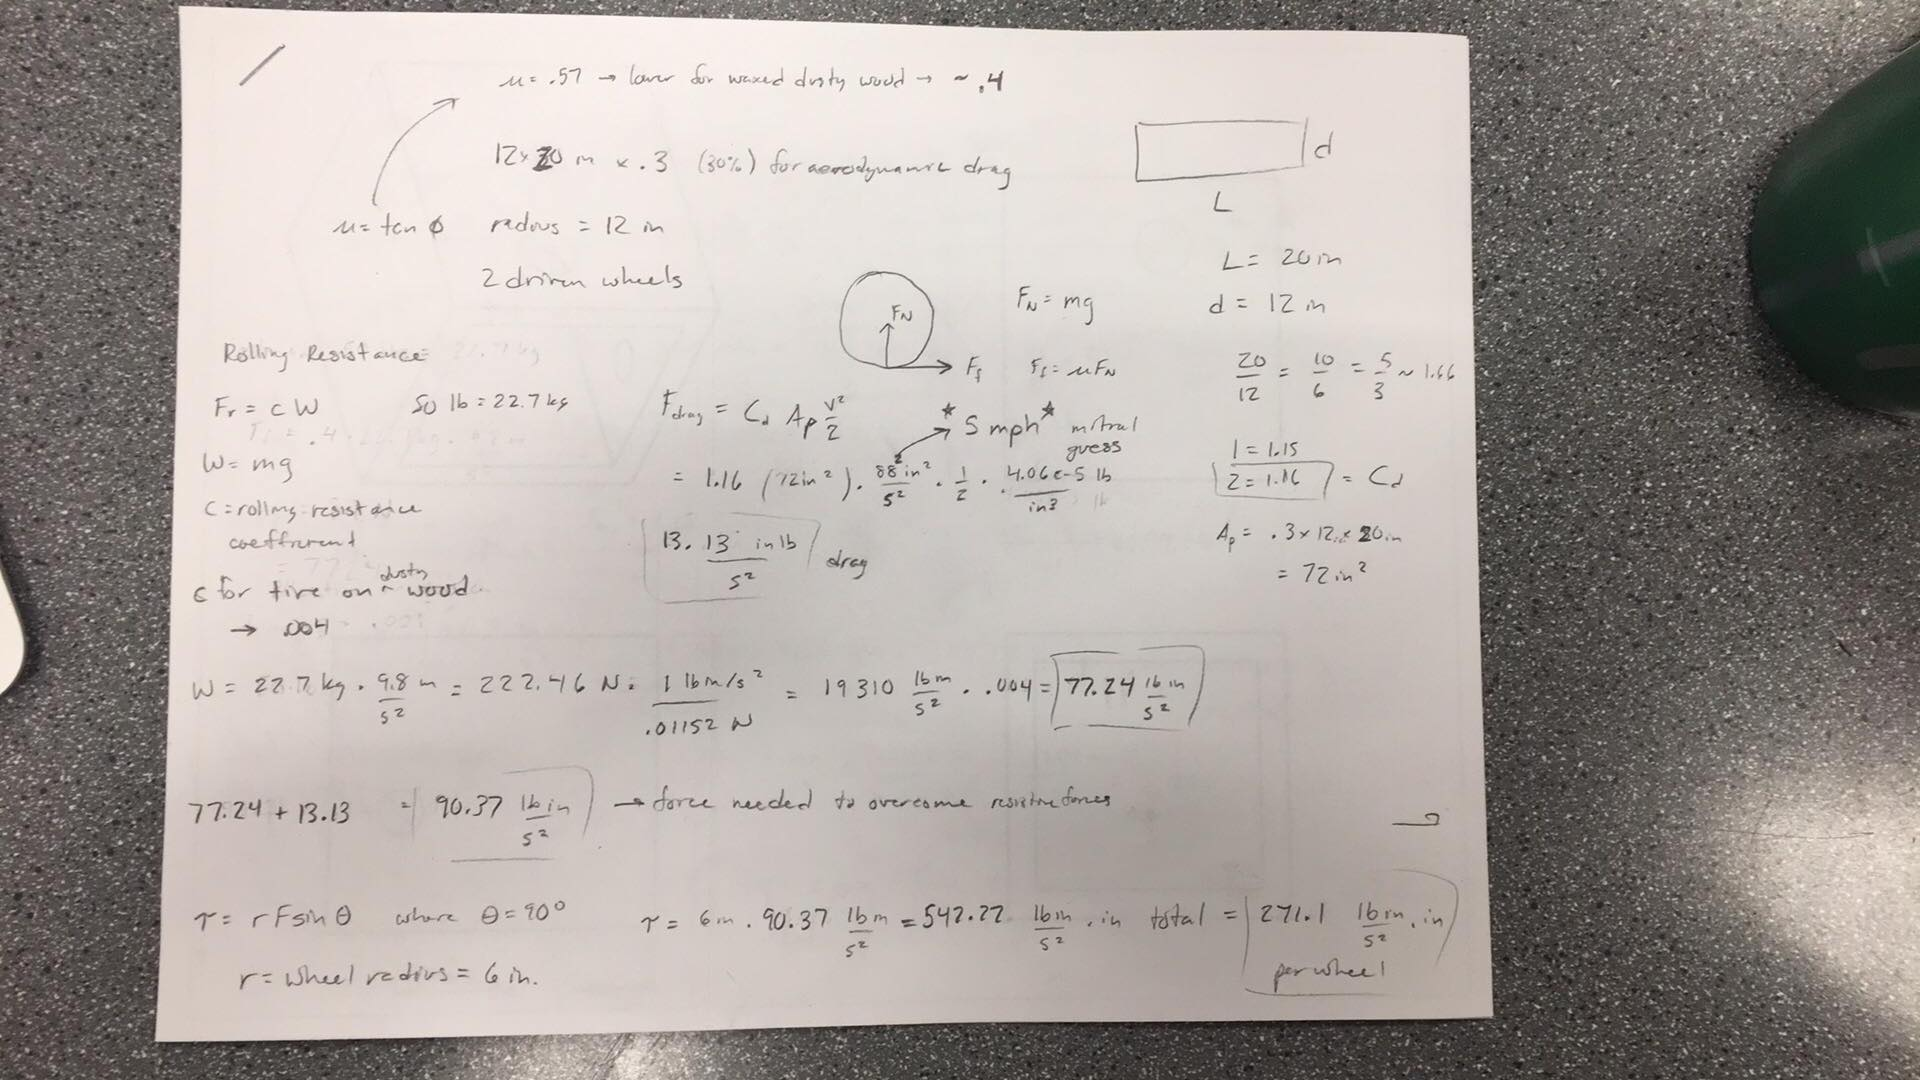
\includegraphics[width=1.1\linewidth]{PreliminaryDesignReport/calculations1.png}
    \caption{Numerical Values and Solutions, part I}
    \label{fig:my_label}
\end{figure}

\begin{figure}[H]
    \centering
    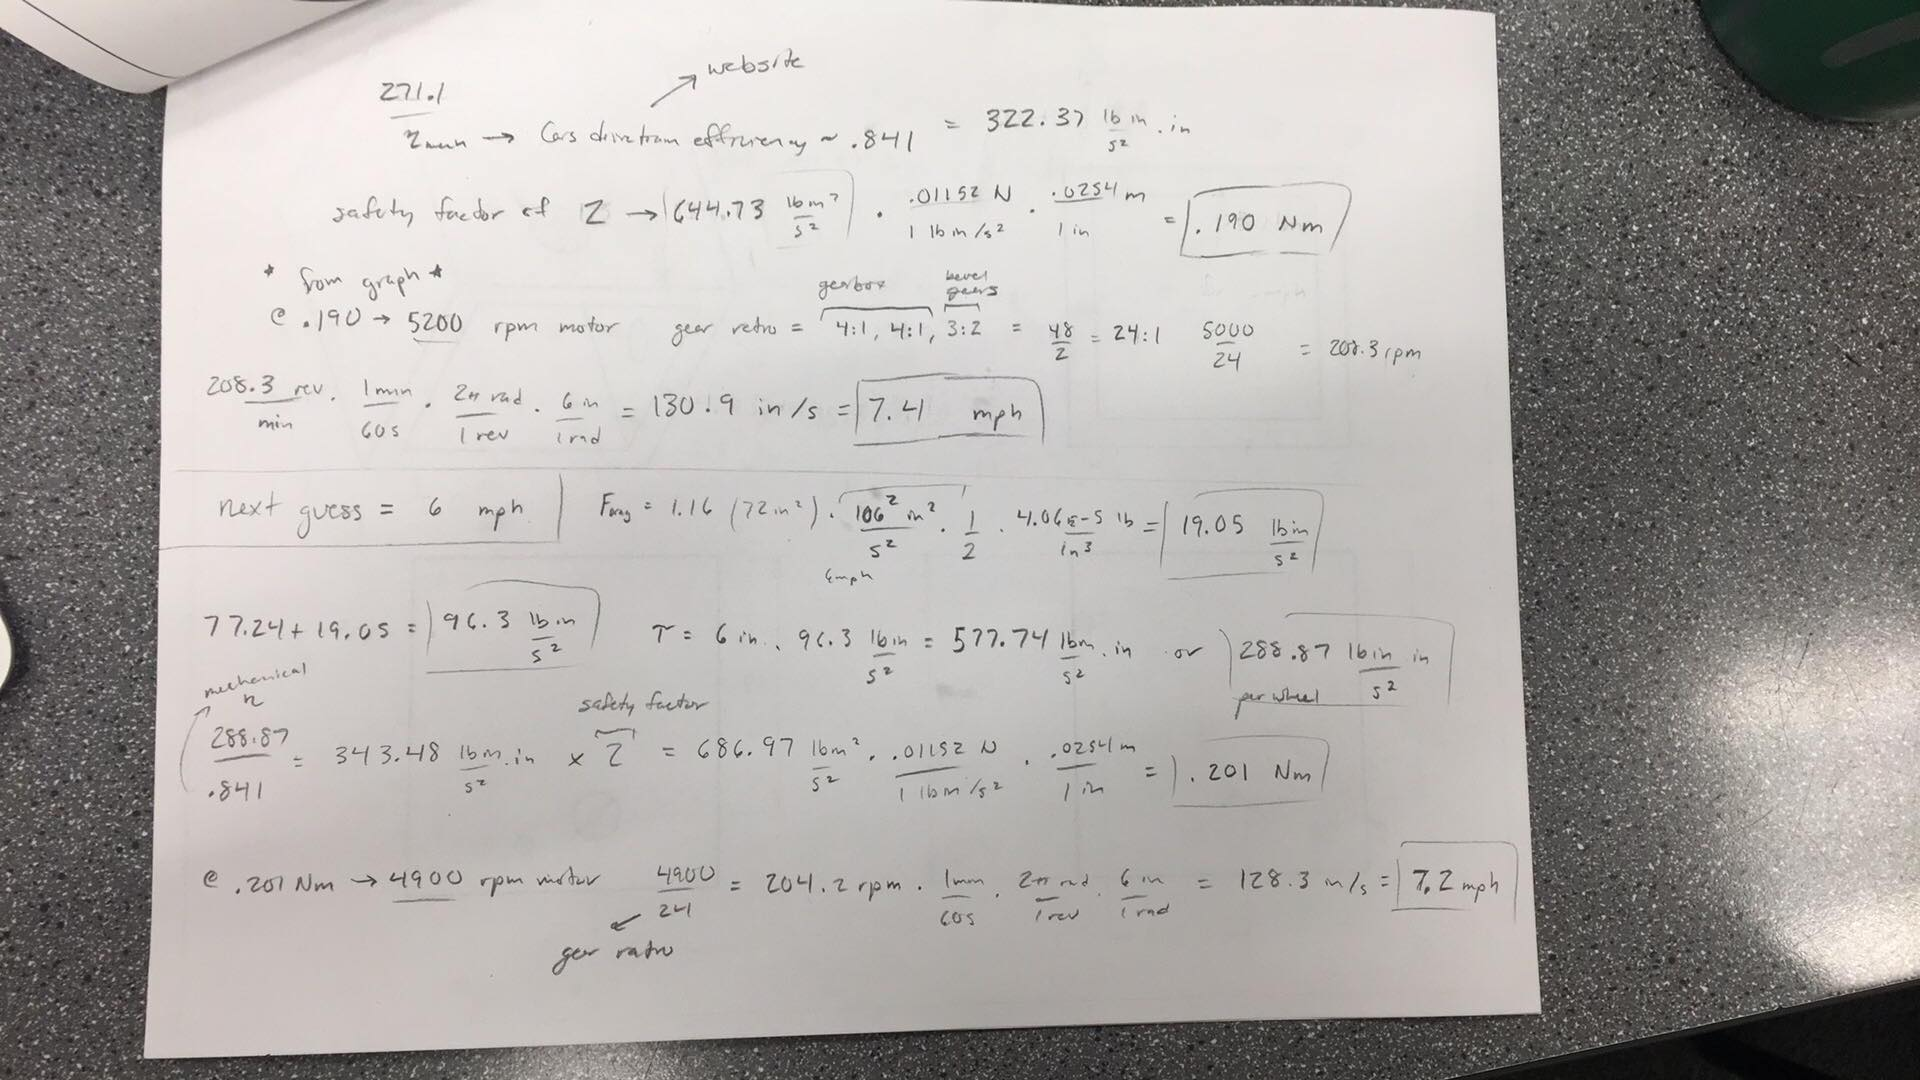
\includegraphics[width=1.1\linewidth]{PreliminaryDesignReport/calculations2.png}
    \caption{Numerical Values and Solutions, part II}
    \label{fig:my_label}
\end{figure}

\begin{figure}[H]
    \centering
    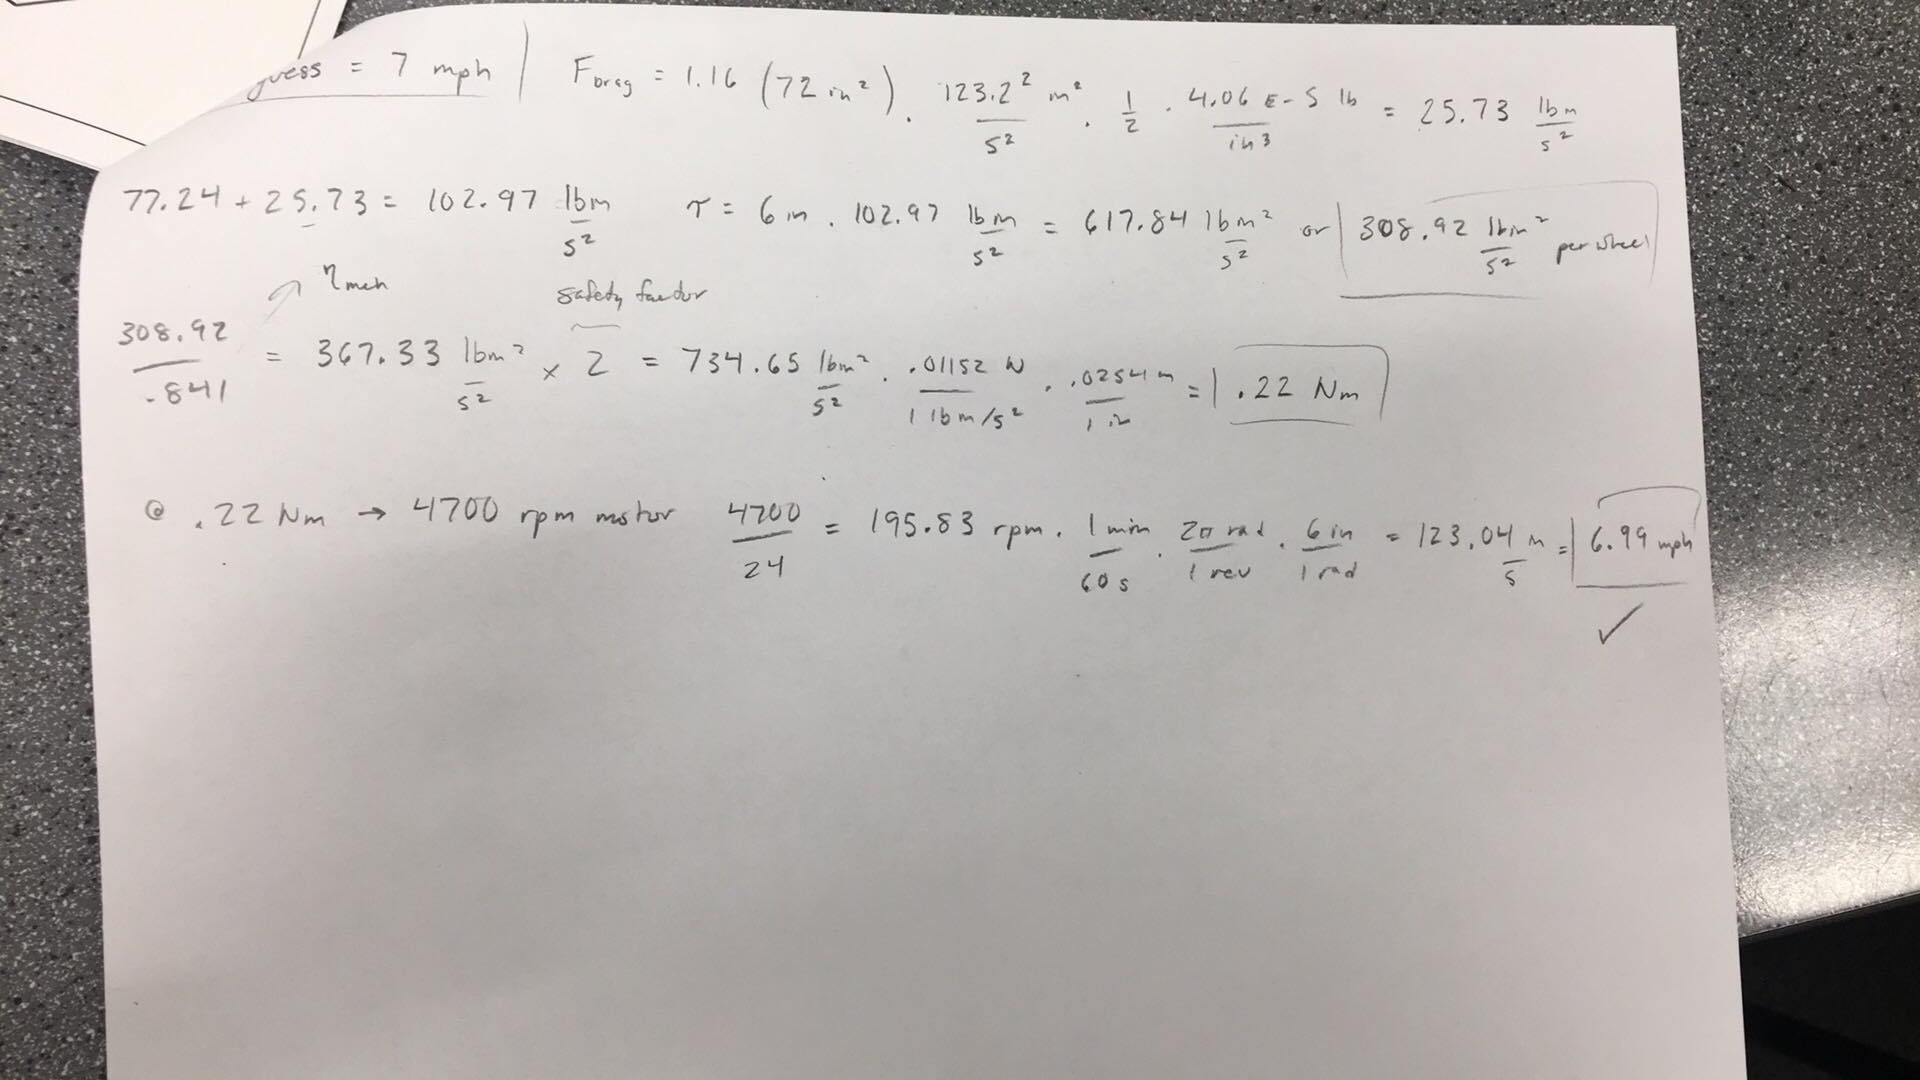
\includegraphics[width=1.1\linewidth]{PreliminaryDesignReport/Calculations3.png}
    \caption{Numerical Values and Solutions, part III}
    \label{fig:my_label}
\end{figure}


\begin{figure}[H]
    \centering
    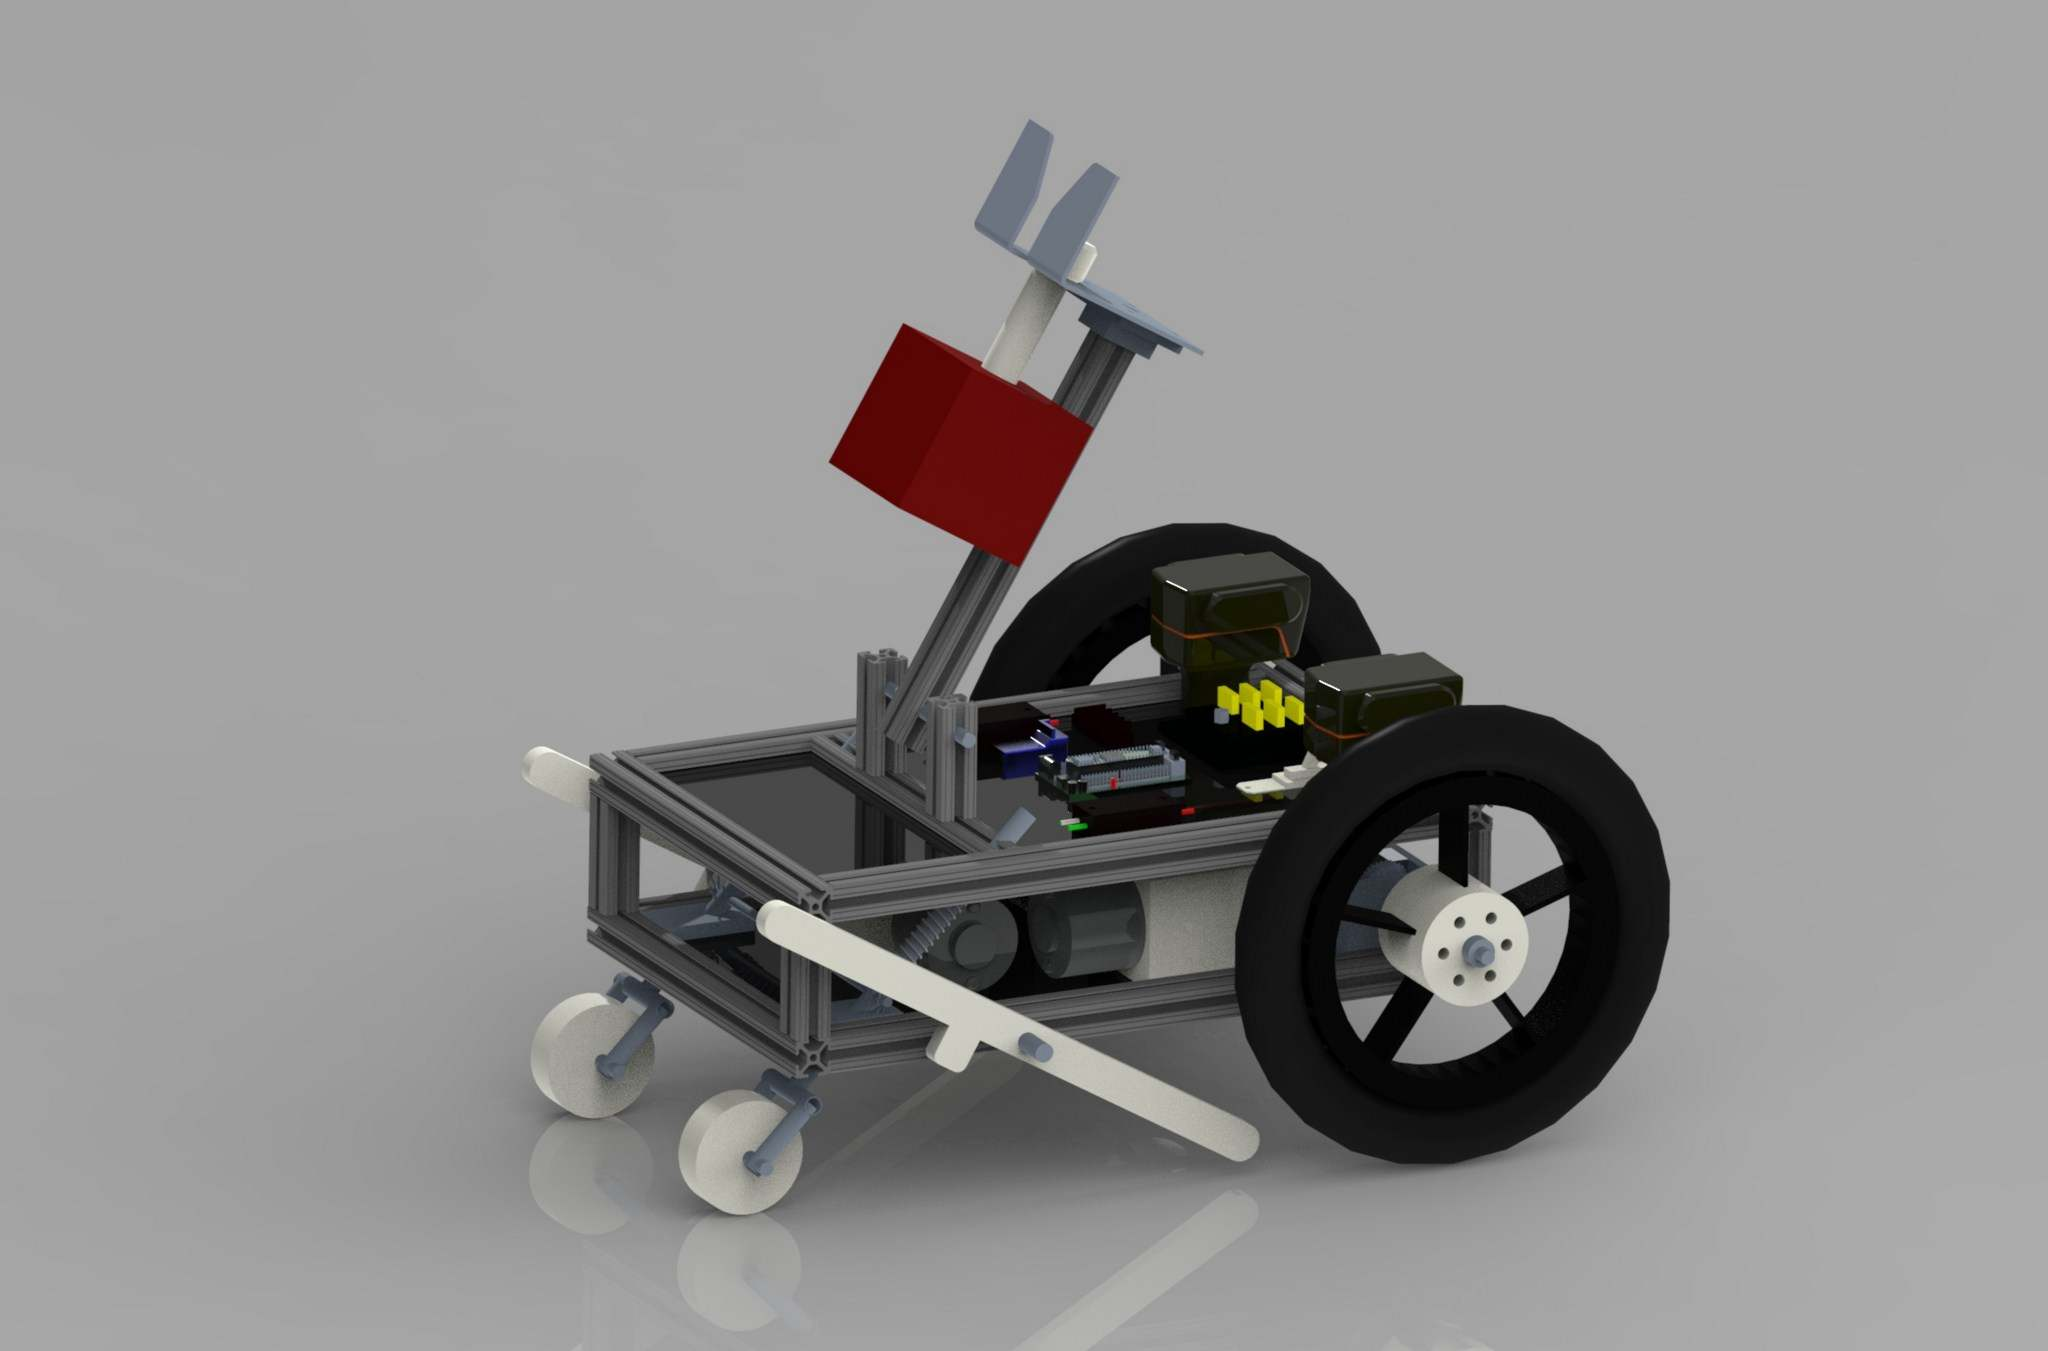
\includegraphics[width=1.2\linewidth]{PreliminaryDesignReport/56306747_2205376912890263_6073389682769526784_n.png}
    \caption{Medical Kit Arm}
    \label{fig:my_label}
\end{figure}




\end{document}